\subsection{3 Sites Results}

We first examine the impact of diversions with a 60 minute
lead time. Figure \ref{fig:3sites_extreme} shows how extreme
waiting cases are reduced. The first thing to notice is that
different sites, when no patients volunteer, and hence our
policy has no effect, already perform quite differently. This is caused by
the different number of machines at each site. York Ave. has 4 machines,
and so it already enjoys substantial pooling effect. This is why patients
generally wait less there. However, as we can see in Figure \ref{fig:3sites_extreme},
diversions reduce extreme waiting cases for all sites, most
prominently at sites with fewer machines.

Since we are optimizing the $L_2$-norm of the waiting time vector,
it is understandable that we can reduce extreme waiting time,
potentially by increasing waiting time for other patients.
Hence, it is interesting to look at how we are doing with respect to mean waiting
time.

\begin{figure}[htp]
\centering
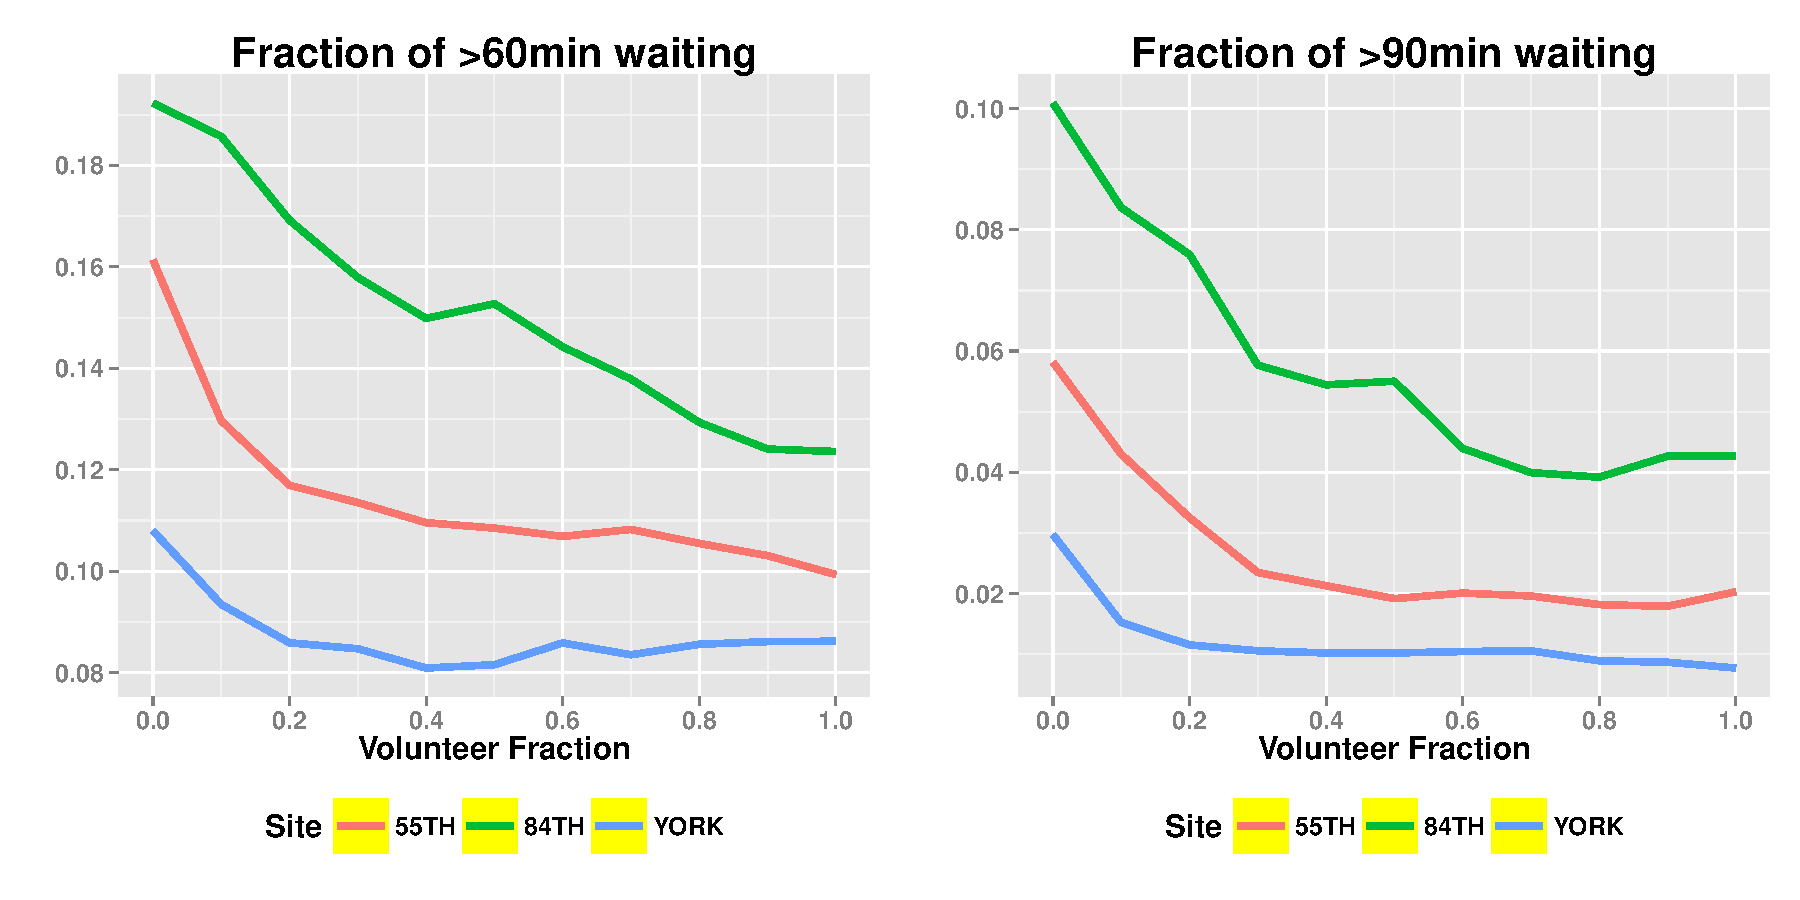
\includegraphics[width=.95\textwidth]{chap3/numeric/pic/3sites_extreme}
\caption{The impact on extreme waiting by diversions.}
\label{fig:3sites_extreme}
\end{figure}

Figure \ref{fig:3sites_wait_over} shows that we actually
reduced mean waiting time for all sites and the reduction
for 84th St and 55th St is again quite significant.
Not only that, we also reduced mean overtime for all sites, and so
the staff can go home earlier. This means that we can finish
the same amount of work within a shorter amount of working time.

\begin{figure}[htp]
\centering
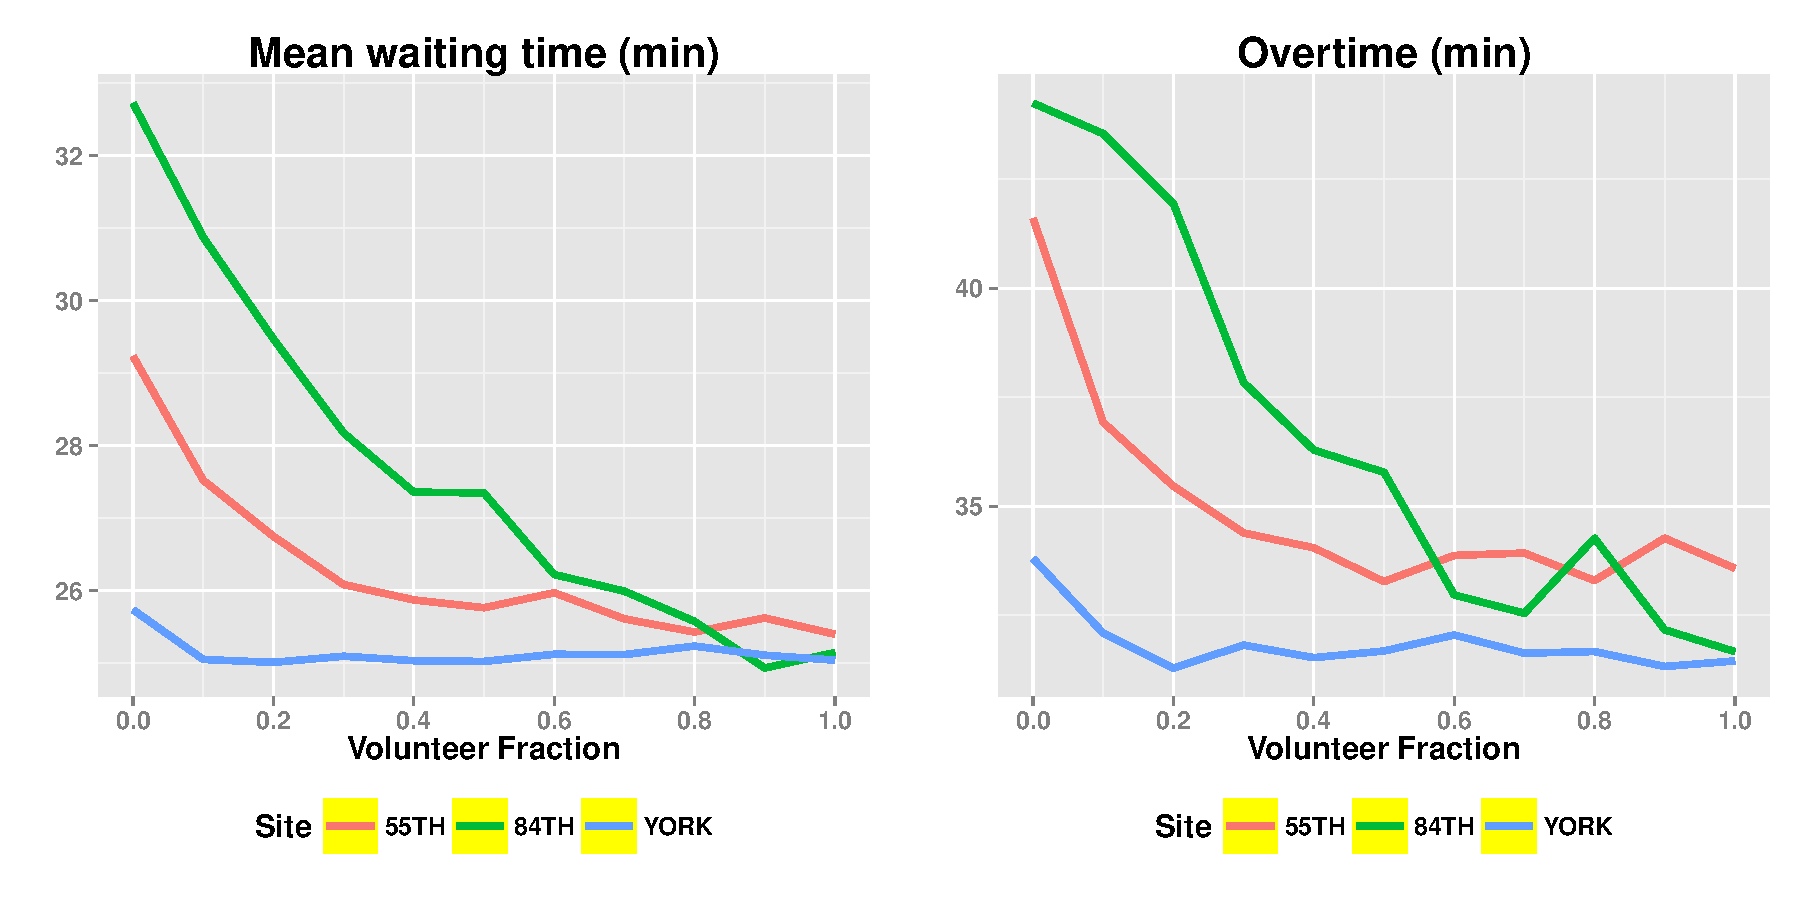
\includegraphics[width=.95\textwidth]{chap3/numeric/pic/3sites_wait_over}
\caption{The impact on mean waiting times and mean site overtimes by diversions.}
\label{fig:3sites_wait_over}
\end{figure}

The explanation for why all three of these metrics improve
can be seen in Figure \ref{fig:3sites_idle}. By
diverting patients to a non-congested site, we actually reduce
idle time there. Because we have made use of some machine time that
would be otherwise wasted in idling, we can finish more work
in the same amount of time, resulting in less backlog and congestion.

\begin{figure}[htp]
\centering
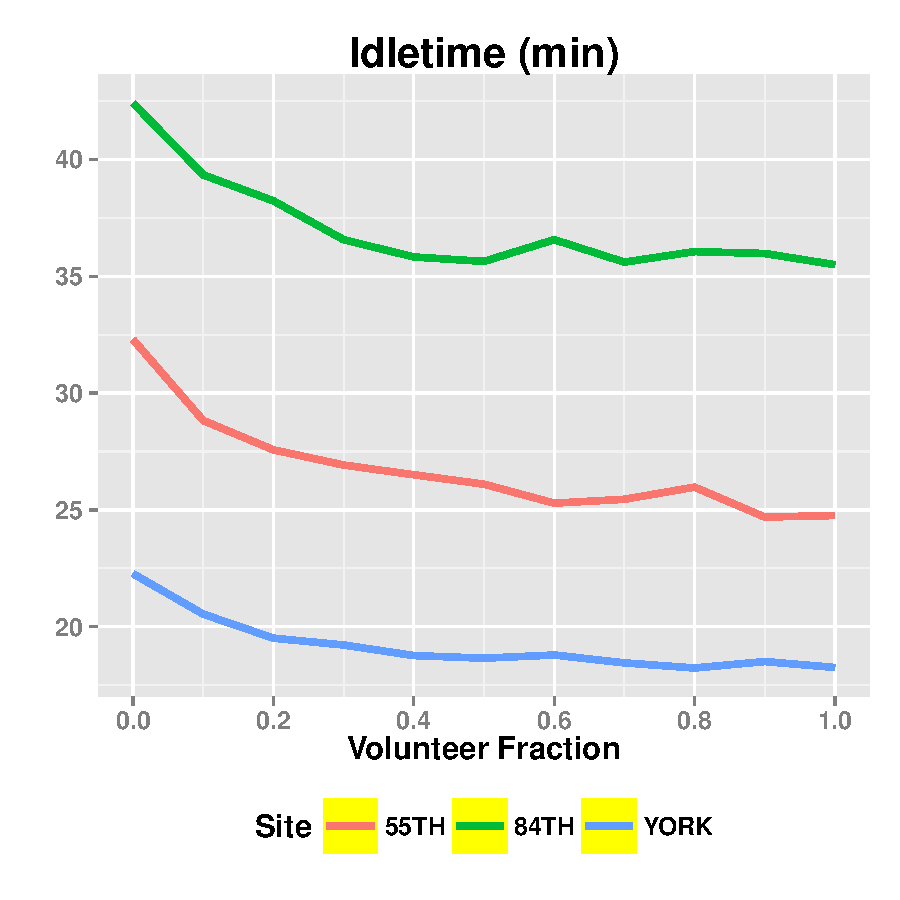
\includegraphics[width=.6\textwidth]{chap3/numeric/pic/3sites_idle}
\caption{The impact on mean idle times.}
\label{fig:3sites_idle}
\end{figure}

Figure \ref{fig:3sites_gain_flow} shows that the most diversions are
made diverting a patient into York Ave, and patients who are diverted into York Ave.
enjoy the greatest reduction in waiting time. This is quite intuitive since
the pooling effect at York Ave. gives it more processing capability.
Consequently, it has more slack to take in additional patients than the other two
sites have. It is important to note that no matter which site the patient is diverted to,
he always enjoys significant reduction in waiting time: this
should serve as great incentive for patients to volunteer provided that they
have the flexbility.

\begin{figure}[htp]
\centering
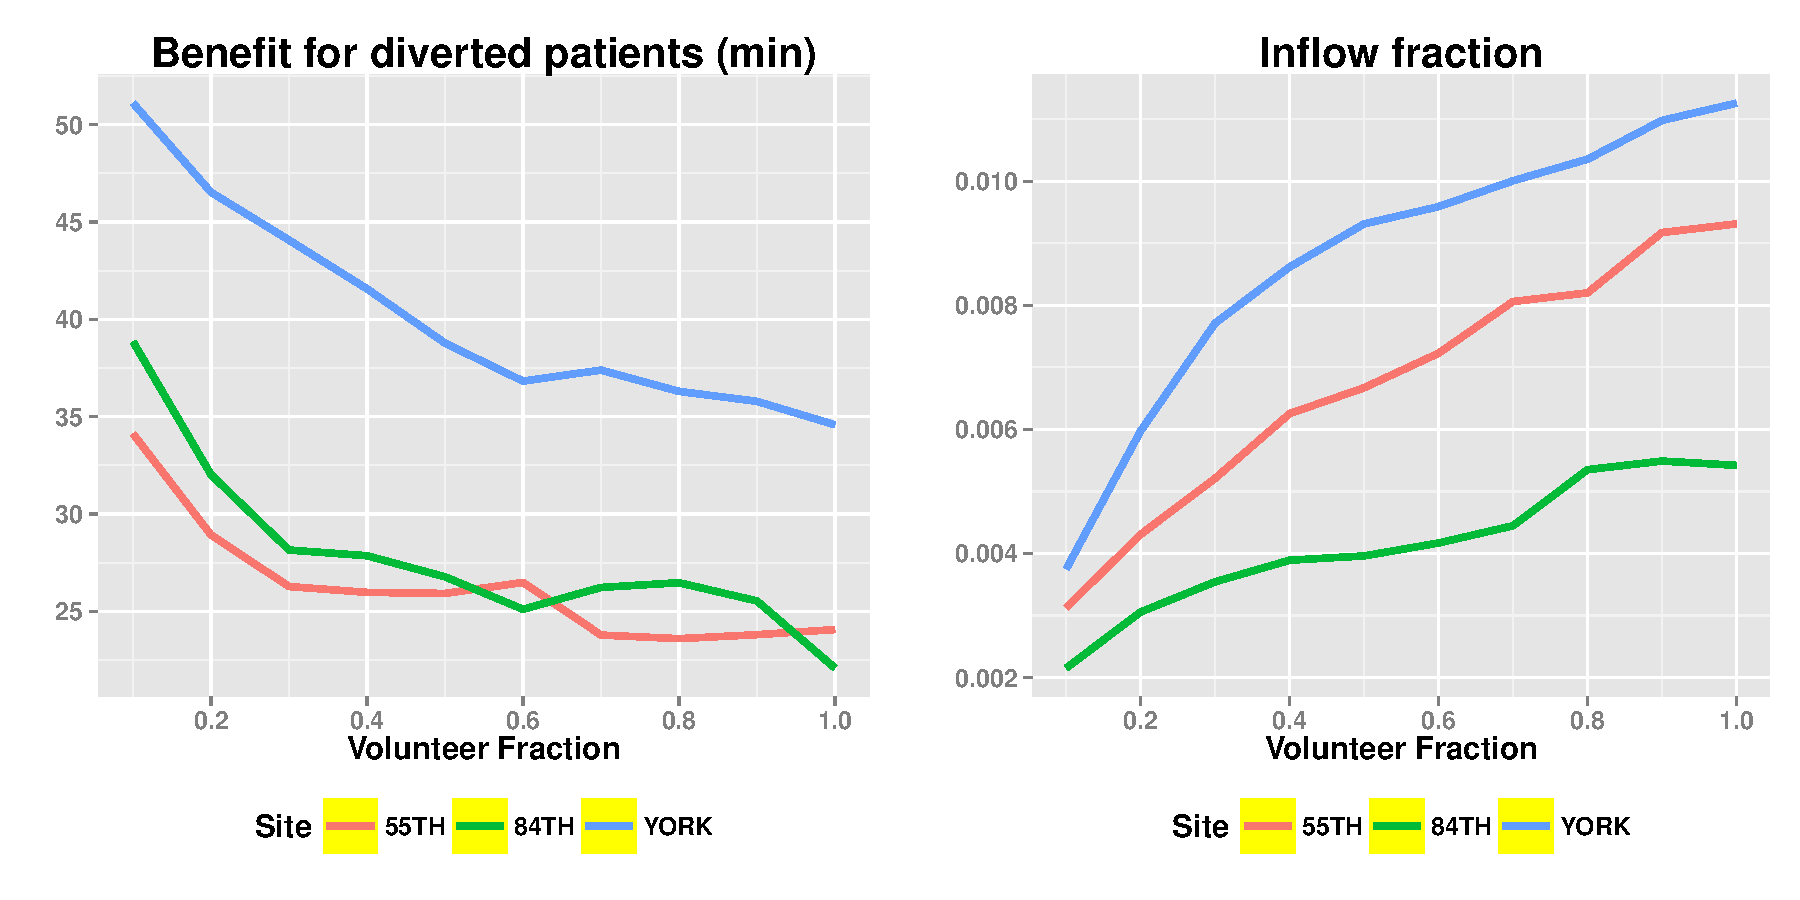
\includegraphics[width=.95\textwidth]{chap3/numeric/pic/3sites_gain_flow}
\caption{The amount of diversion into each site and reduction of waiting time
enjoyed being diverted into each site.}
\label{fig:3sites_gain_flow}
\end{figure}

Overall, we can see across all the figures, that the system performance
improves fastest when we only have very small fraction of patients as
volunteers. In other words, diversions can rapidly improve system
performance with very little flexbility. This is desirable since
benefits seen in a limited trial can give then practioner more confidence
to implement this more broadly.

Figure \ref{fig:3sites_all} shows the overall system performance for both a 60 minute
lead time and a 90 minute lead time cases. The results closely mimic the
discussion above. Overall, with a 60 minute lead time and 40\% volunteers,
we reduce the fraction of over 60 minute waitings from 13.5\% to 9.7\%, and the fraction of
over 90 minute waitings from 4.7\% to 1.8\%. Both overtime and idle time
are also significantly improved.

However, we would like to stress that even with a 90 minute lead time, the diversions
still bring much improvement, and indeed not that different from
the performance with a 60 minute lead time. This has a quite important practical
implication, since a longer lead time makes it easier for patients to be
diverted to different sites.

\begin{figure}[htp]
\centering
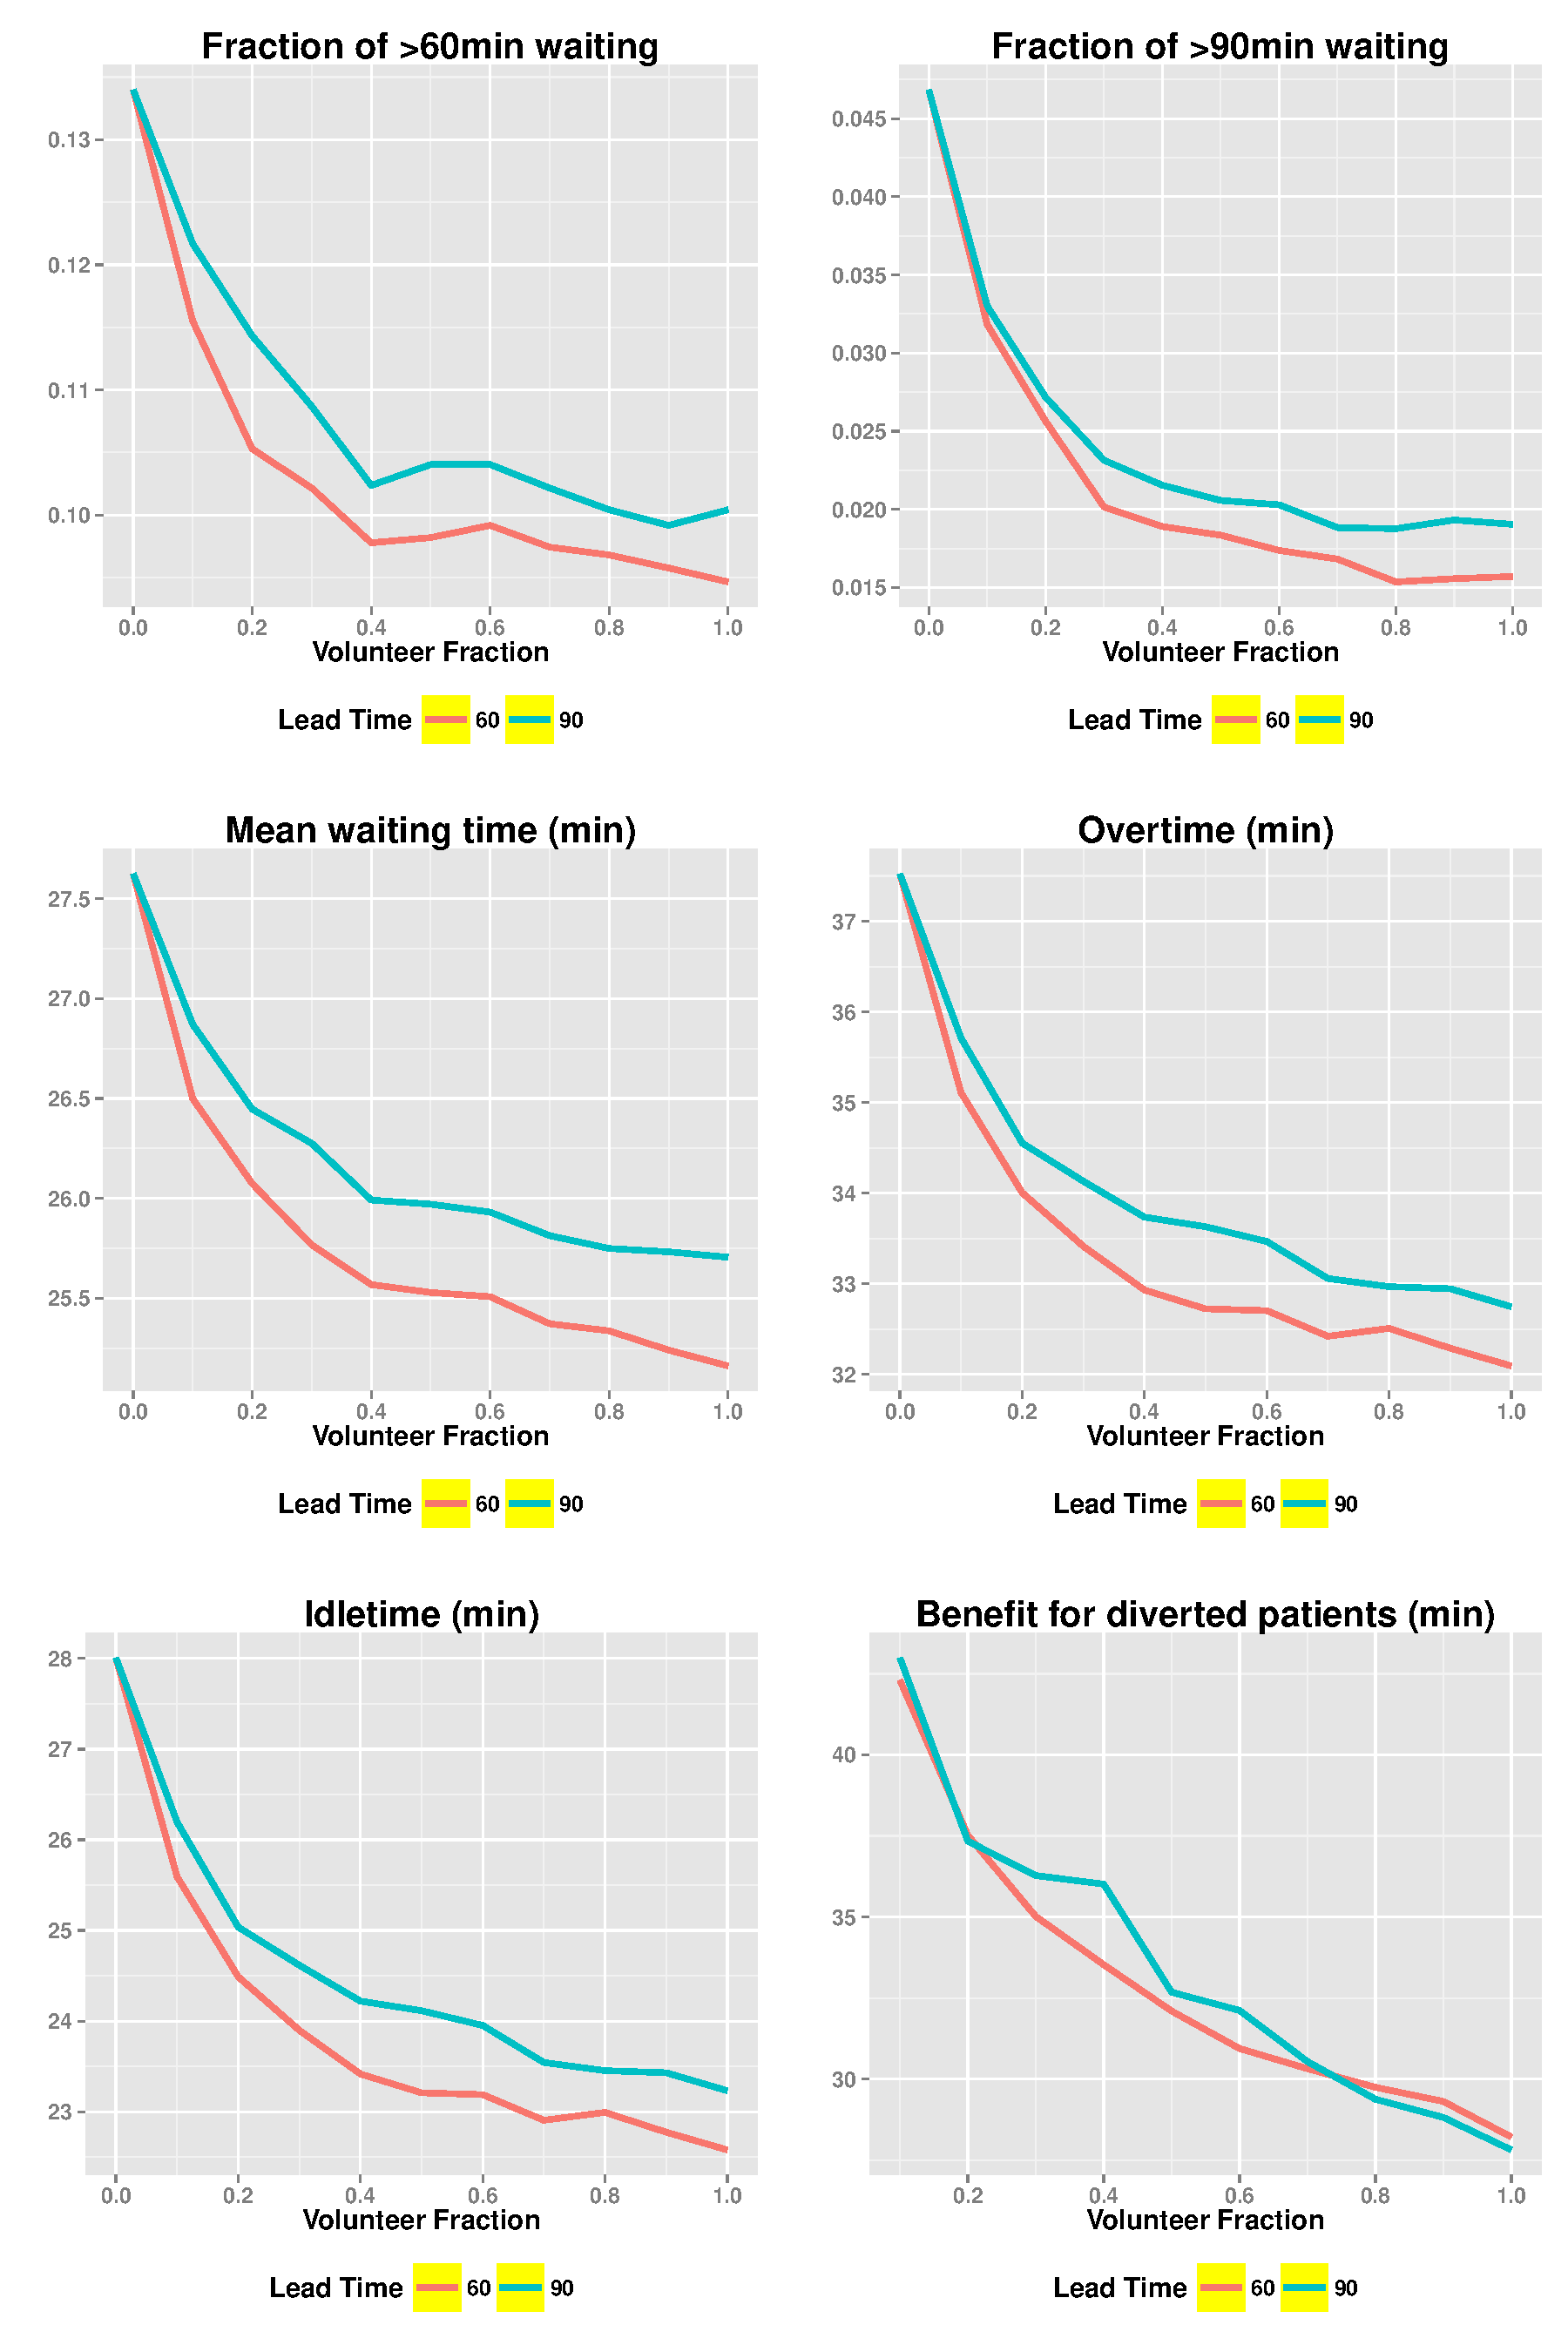
\includegraphics[width=.95\textwidth]{chap3/numeric/pic/3sites_all}
\caption{System performance improvement by diversion.}
\label{fig:3sites_all}
\end{figure}

We also want to note that, as Figure \ref{fig:3sites_all_diversion} shows,
we only diverted a very small fraction of the patients. Even if all patients
are volunteers, we only diverted fewer than 3\% of them.
We believe that this is a desirable property, since fewer changes are easier
to implement. Also, since there are only 3 changes per day on average,
the staff can use their domain knowledge to better facilitate those
changes.

\begin{figure}[htp]
\centering
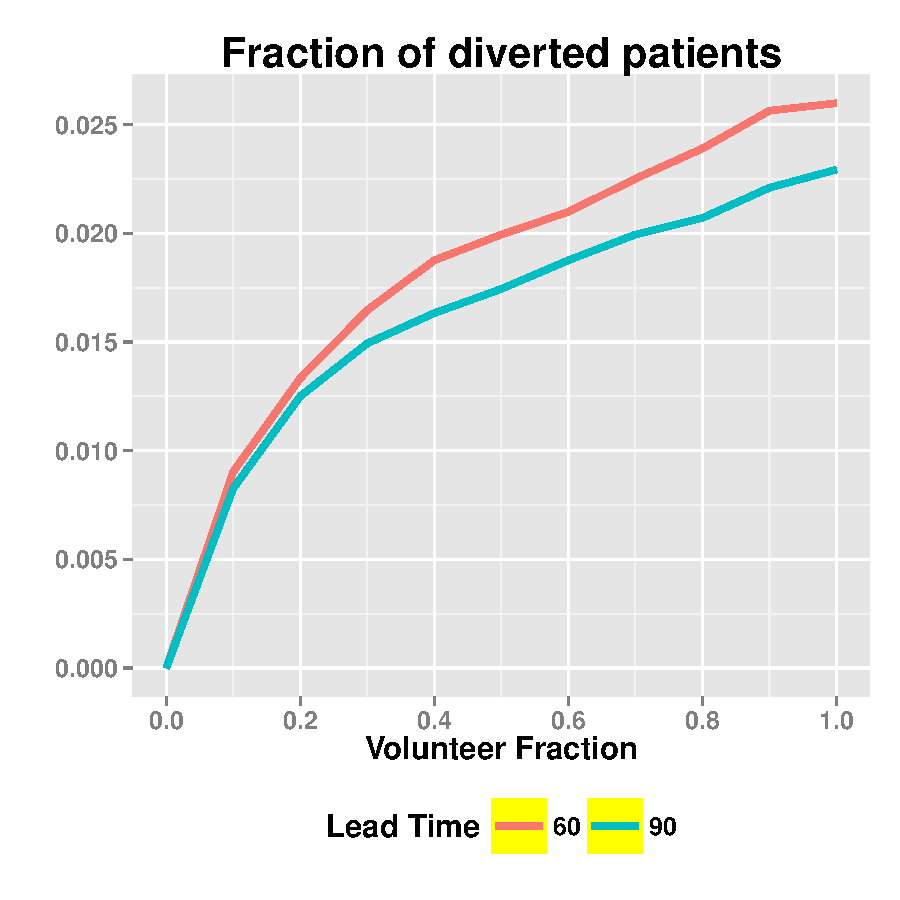
\includegraphics[width=.6\textwidth]{chap3/numeric/pic/3sites_all_diversion}
\caption{Fraction of patients diverted.}
\label{fig:3sites_all_diversion}
\end{figure}

Overall, we think diversions are shown to be an efficient way to
improve system performance for NYP Hospital's outpatient MRI sites.
It can significantly improve patient waiting time and site overtime,
without incurring too many diversions.
